\chapter{Introduction}


\section{Motivation}

\subsection{3D arrays}

Sound propagates in 3D: need for 3D mic arrays to capture spatial properties



\subsection{spherical microphone arrays}

\begin{itemize}
  \item even distribution of capsules
  \item mathematical convenience: spherical harmonics
\end{itemize}



\subsection{ambisonics}


advantages on the vr/ar context
\begin{itemize}
  \item device independent
  \item intermediate storage format
  \item signal-independent transformations are easy
  \item de-facto standard for vr
\end{itemize}

\subsection{Current limitations of vr/ar production}


\section{Goals}

Research question: 	How can we exploit the characteristics of ambisonic recordings in order to manipulate them more adequately? 


\section{Context}

Different levels of application/contribution:

\begin{itemize}
	\item Acoustic Parameter Estimation (low level, audio2data)
	\begin{itemize}
		\item Direction of Arrival estimation
		\item Coherence analysis
		\item Acoustic description (RT60, etc)
		\item Source counting
	\end{itemize}

	\item Signal Enhancement  (high level, audio2audio)
	\begin{itemize}
		\item Source Separation
		\item Dereverberation / denoising
		\item IR estimation
	\end{itemize}

	\item Scene Description (high level, audio2data)
	\begin{itemize}
		\item Event Detection
		\item Acoustic Scene Classification
	\end{itemize}
\end{itemize}

\begin{figure}[hbt]
  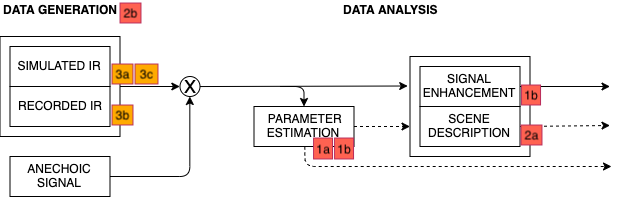
\includegraphics[width=\textwidth]{Figures/Introduction/context_scheme.png}
  \caption{\todo{todo caption}}
\end{figure}


\todo{introduce rest of chapters?}
